\documentclass[letterpaper,12pt]{report}
\usepackage[top=1in, bottom=1in, left=1in, right=1in]{geometry}
\usepackage{fancyhdr,tocloft,natbib,url,graphicx,float,listings,sidecap,wrapfig,setspace,subcaption}
\usepackage[font=small,labelfont=bf,labelsep=period]{caption}
\usepackage{tabularx}
\usepackage{setspace}
\usepackage{hyperref}
\usepackage[all]{hypcap}
\usepackage{qtree,algorithm,algorithmic}
\pagestyle{plain}
\fancyhf{}
\lhead{}
\chead{}
\rhead{}
\cfoot{\thepage}


%\floatstyle{boxed}
%\restylefloat{figure}

\hypersetup {
	colorlinks=false,
	pdfborder={0 0 0},
}

\setcounter{secnumdepth}{3}
\renewcommand*\thesection{\arabic{section}.}
\renewcommand*\thesubsection{\thesection \arabic{subsection}.}
\renewcommand*\thesubsubsection{\thesubsection \arabic{subsubsection}.}

\setcounter{tocdepth}{3}
\renewcommand\contentsname{}				% TOC title
\renewcommand\listfigurename{}				% LOF title
\renewcommand\listtablename{}				% LOT title
\renewcommand{\baselinestretch}{1.5}
\setlength\cftaftertoctitleskip{-0.5in}
\setlength\cftafterloftitleskip{-0.5in}
\setlength\cftafterlottitleskip{-0.5in}

\renewcommand\bibsection{\section{References}}

\begin{document}

\hypersetup{pageanchor=false}
%%  COVER PAGE
\begin{titlepage}
	\begin{center}
		\vspace*{0.5in}
		\begin{doublespace}
			\LARGE \textbf{Giftbox} \\
			\vspace*{1in}
			\normalsize
			A Manuscript \\
			Submitted to \\
			the Department of Computer Science \\
			and the Faculty of the\\
			University of Wisconsin--La Crosse \\
			La Crosse, Wisconsin \\
			\vspace*{0.5in}
			by \\
			\large
			\textbf{Siyan Ding} \\

			\vspace*{0.5in}
			\normalsize
			in Partial Fulfillment of the \\
			Requirements for the Degree of\\
			\Large{\textbf{Master of Software Engineering}} \\
			\normalsize
			December, 2018
		\end{doublespace}
	\end{center}
\end{titlepage}
	
\clearpage

%% SIGNATURE PAGE
\thispagestyle{empty}
\vspace*{0.3in}
\begin{center}
	\large{\textbf{Giftbox}} \\ 
	\vspace{0.75in}
	\normalsize{By Siyan Ding}
\end{center}

\vspace{0.5in}
\noindent We recommend acceptance of this manuscript in partial fulfillment of this candidate's requirements for the degree of Master of Software Engineering in Computer Science. The candidate has completed the oral examination requirement of the capstone project for the degree. \\

\noindent
\begin{tabularx}{\textwidth}{p{3in}Xp{2in}}
	\rule{0pt}{50pt} & & \\
	\hrulefill & & \hrulefill \\
	Prof. Kenny Hunt & & Date \\
	Examination Committee Chairperson & & \\
	\rule{0pt}{50pt} & & \\
	\hrulefill & & \hrulefill \\
	Prof. Kasi Periyasamy & & Date \\
	Examination Committee Member & & \\
	\rule{0pt}{50pt} & & \\
	\hrulefill & & \hrulefill \\
	Prof. Allison Sauppé & & Date \\
	Examination Committee Member & & \\
\end{tabularx}


\clearpage

\hypersetup{pageanchor=true}
\setcounter{page}{1}
\pagenumbering{roman}
\renewcommand\arraystretch{1.5}

%% ABSTRACT
\section*{Abstract}
\addcontentsline{toc}{section}{Abstract}
Mai, Diep, H., ``Object-Z-Based Test Case Generator,'' Master of Software Engineering, May 2011, (Kasi Periyasamy, Ph.D.). \\

This manuscript describes the development of a specification-based test case generator following the model-based testing methodology. Model-based testing is performed based on the testing models derived from a system under test. This test case generator reads the Object-Z specification modeling a testing model from the command line and employs the boundary value analysis technique to generate test cases for the model. All test cases are categorized to valid and invalid set. In addition, the tool can also be used to verify the inconsistency and ambiguity in a specification.
\clearpage

%%% ACKNOWLEDGEMENTS
\section*{Acknowledgements}
\addcontentsline{toc}{section}{Acknowledgments}
I would like to express my sincere appreciation to my project advisor Dr. Kasi Periyasamy for his invaluable guidance and untiring support. I would also like to express my thanks to the Department of Computer Science at the University of Wisconsin--La Crosse for providing the learning materials and computing environment for my project.
\clearpage

%% TABLE OF CONTENTS
\section*{Table of Contents}
\tableofcontents
\clearpage


%% LIST OF TABLES
\section*{List of Tables}
\addcontentsline{toc}{section}{List of Tables}
\listoftables
\clearpage

%% LIST OF FIGURES
\section*{List of Figures}
\addcontentsline{toc}{section}{List of Figures}
\listoffigures
\clearpage

%% GLOSSARY
\section*{Glossary}
\addcontentsline{toc}{section}{Glossary}


\subsubsection*{API}

A set of routine definitions, protocols, and tools for building software and applications. An API specification can take many forms, but often include specifications for routines, data structures, object classes, or variables.

\subsubsection*{AR}

Augmented reality is the integration of digital information with the user's environment in real time. Unlike virtual reality, which creates a totally artificial environment, augmented reality uses the existing environment and overlays new information on top of it.

\subsubsection*{CSRF}

Cross-site request forgery, also known as one-click attack or session riding and abbreviated as CSRF or XSRF, is a type of malicious exploit of a website where unauthorized commands are transmitted from a user that the web application trusts.\cite{Ristic2005}

\subsubsection*{Function as a Service}

Function as a service (FaaS) is a category of cloud computing services that provides a platform allowing customers to develop, run, and manage application functionalities without the complexity of building and maintaining the infrastructure typically associated with developing and launching an app.\cite{roberts_2018}

\subsubsection*{GPS}

The Global Positioning System (GPS), originally Navstar GPS, is a satellite-based radio navigation system owned by the United States government and operated by the United States Air Force.[2] It is a global navigation satellite system that provides geolocation and time information to a GPS receiver anywhere on or near the Earth where there is an unobstructed line of sight to four or more GPS satellites.

\subsubsection*{GUI}

A graphical user interface utilizes the graphical capabilities of a computer to provide a
user interface for computer software. GUIs often employ images, symbols and visual cues
to facilitate user interaction in a point-and-click manner. Common methods for providing
user input include the use of keyboards, mice, pen devices, touch screens or other devices
for physical interaction.

\subsubsection*{Open Source Software}

Open Source Software (OSS) is software distributed with a license allowing access to its
source code, free redistribution, the creation of derived works, and unrestricted use.

\clearpage

\setcounter{page}{1}
\pagenumbering{arabic}

\IfFileExists{section01/section}{\section{Introduction}
\label{sec:Introduction}

\subsection{Overview} 
\paragraph{}
Ours is an increasingly visual culture and with the development of computing technology, people are no longer simply satisfied with just the visible but have a higher demand of visual effects.
% AR or image process
\par Augmented Reality (AR) is a strong and emerging presence in the IT market. Enhanced GPS systems are using AR to make it easier to get from point A to point B. The ability to augment a live view of displays in a museum with facts and figures is a natural use of the technology as well. With recent advances in computing power and technology, gaming applications with digital image processing are on the upswing, too. Head mounted systems are inexpensive and computing power is more portable than ever. 
\par Evidently, AR, an advanced technology, has furthered and enhanced several aspects of our life and the technology behind is really meaningful.

\subsection{Motivation}
\paragraph{}
In July 2016, an AR mobile game named Pokemon Go was released in certain countries, and in other regions over the next few months. The game uses the mobile devices GPS to locate, capture, battle, and train virtual creatures, called Pokemon, which are projected onto the camera in real-time to appear as if they are in the player's real-world location. 
\par
The game was referred to as a "social media phenomenon" which has brought people together from all walks of life.\cite{duffy_2016} \cite{kain_2016} Over 231 million people engaged in 1.1 billion interactions that mentioned Pokemon Go on Facebook and Instagram in the month of July.\cite{laurenjohnson_2016} Numerous media outlets referred to the surge in popularity as "Pokemon Go Mania", or simply "Pokemania".\cite{isaac_2016} \cite{steinmetz_2016} The massive popularity of the game resulted in several unusual positive effects. For example, the game enabled players to help catch criminals and to report crimes in progress,\cite{daye_2016} \cite{reports_2016} \cite{staff} and has even aided law enforcement's community relations,\cite{cherelus_2016} albeit with caveats.\cite{rocha_2016} Businesses also benefited from the nearby presence of PokeStops (or them being PokeStops themselves) with the concomitant influx of people,\cite{shields_perlberg_2016}\cite{sydneyShaw_2016} and the intense exploration of communities has brought local history to the forefront.\cite{butcher_2016} The game was also seen bringing its players to places of worship, as many Pokegyms are located there.\cite{ahmed_2016} Despite some criticism by religious leaders, this was received positively by religious groups, who saw it as reminding adherents to come and pray.\cite{r_2016}
\par
Pokemon Go was one of the most used and profitable mobile apps in 2016, having been downloaded more than 500 million times worldwide by the end of the year. It is credited with popularizing location-based and AR technology, promoting physical activity, and helping local businesses grow due to increased foot traffic. In May 2018, The Pokemon Company announced that the game had received over 800 million downloads worldwide, and it has 147 million monthly active users as of May 2018. As of September 2018, the game has grossed 2.01 billion dollars worldwide.

\subsection{The Gift Box Application}
\paragraph{}
This application seeks to explore the augmented-and-virtual-reality space by creating an Android app that allows users to attach virtual messages or objects at specific places in the real world. Virtual entities will be viewable and recoverable only by those individuals that the user selects. The locations of these objects are determined by a combination of GPS coordinates in conjunction with image processing keypointing.
\par Imagine a user with a mobile Android device. The user walks into a room and takes an image of a wall-hanging, as shown in Figure 1(a). The app allows the user to select a place in the image to which a virtual entity can be attached. This selection process can be partially automated. The user then selects a virtual object offered by the application or create one themselves. The virtual object will be later send to the recipient chosen by the user. Recipients are notified that a virtual gift has been granted to them and they are only given the location of that object. Each recipient must then navigate to the same room, scan the room with their app, and if they scan the targeted room region, they will receive the virtual gift. A mock-up of the gifting process is shown in Figure 1(b).

\begin{figure}[H]
\centering
\begin{minipage}[t]{0.5\textwidth}
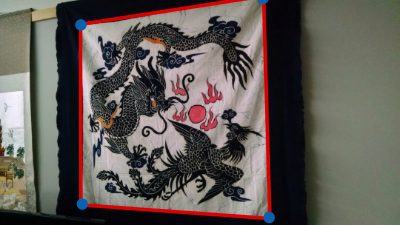
\includegraphics[width=.95\textwidth]{section01/assets/giftbox_1.png}
\subcaption{}
\end{minipage}%
\begin{minipage}[t]{0.5\textwidth}
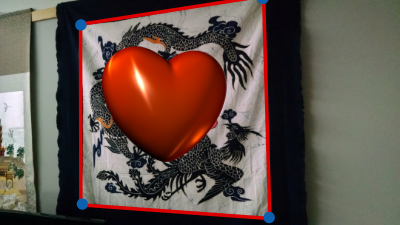
\includegraphics[width=.95\textwidth]{section01/assets/giftbox_2.png}
\subcaption{}
\end{minipage}%
\caption[Short Caption]{Example Result}
\end{figure}

\paragraph{} This application also contains a web interface that allows user to have a general idea of the whole project before they download the android application. Users can not only view and edit their profile but also manage their friends list online. If you don't have your Android device with you it will be a good choice to check if you have any recently received gifts online as well. At the same time, it leaves an interface for administrator users to add more virtual gifts into the database and manage user activities.



}{}\clearpage
\IfFileExists{section02/section}{\section{Requirements}
\label{sec:Requirements}



%openCV, bmob
\subsection{Overview} 
\label{RequirementsOverview}
\paragraph{}
The Gift Box Project was conceived by Dr. Hunt inspired by the very popular game Pokemon Go. For this project, Dr. Hunt served as the supervisor and the sponsor.
\par The supervisor met with the developer several times to gather informal functional requirements of this program. These informal functional requirements helped to define the scope of the program as well as capture the true nature and purpose of the application. During the first of these informal meetings, the supervisor provided samples of the processed pictures with a wall-hanging and identified how to select a region. Based on the information collected from these meetings, the requirement document version 1.0 was created, in which the following requirements were listed:
\begin{itemize}
\item This project will support both a web interface and an Android application.
\item The gifts sent by a user can be selected from a pre-defined library or created by users. 
\item The gift will be projected onto the region chosen by user.
\item GPS navigation allows users to find gifts but it only supports 2D locations. 
\item The application will attempt to robustly allow gifts to be found from a variety of angles, distances, and lighting conditions.
\end{itemize}
\par The project initially included the development of the image comparator which include image recognition and image transformation algorithms. However, the scope of the image comparator was too large and imposed too much complexity on the developer. To address this complexity, the developer, with assistance from Dr. Hunt, decided to use third-party software packages which would be able to perform the functionalities of image recognition. A software package was chosen depending on the required features. The scope of the program was therefore appropriately reduced by using the third-party software for the complex image recognition.
\par The detailed functional requirements are described in Section \ref{FunctionalRequirements} Functional Requirements. 

\subsection{Functional Requirements}
\label{FunctionalRequirements}
\paragraph{}
This program only supports one role, the System User for Android Application. Figure \ref{Use Cases Diagram} gives a Use Case diagram for the System User.
\par As shown in the Figure \ref{Use Cases Diagram}, there are eight use cases in the diagram. Each use case describes a functional requirement. These functional requirements are narrated as follows:

\begin{figure}[htb]
\centering
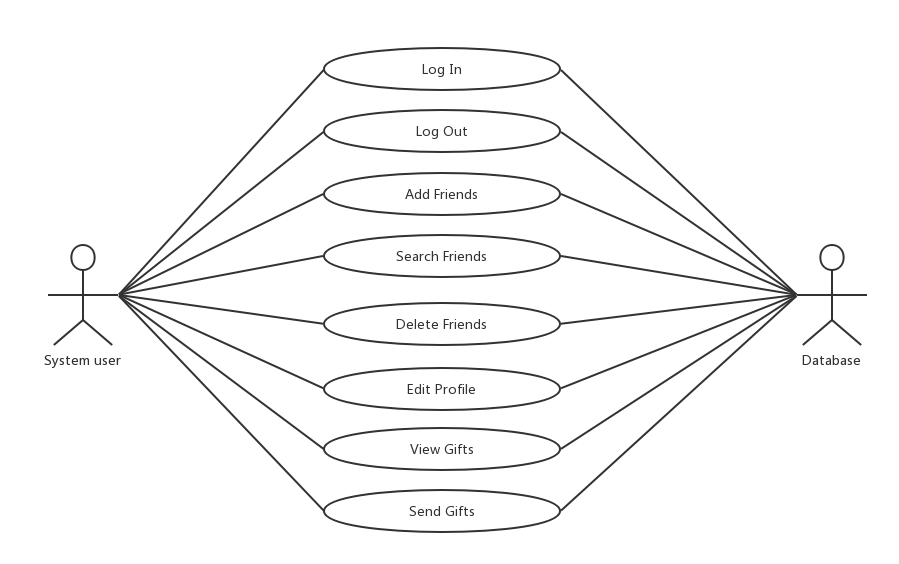
\includegraphics[width=.5\textwidth]{section02/assets/UseCase.png}
\caption[Use Case Diagram for Android Application]{\label{Use Cases Diagram}Use Case Diagram for Android Application}
\end{figure}

\begin{itemize}
\item The \bsq{Log In} function allows users to log in to the system.
\item The \bsq{Log Out} function allows users to log out of the system.
\item The \bsq{Add Friends} function allows users to add other users as friends. This add function doesn't need other users' agreement.
\item The \bsq{Search Friends} function allows users to search other users by username.
\item The \bsq{Delete Friends} function allows users to delete friends from their friends list.
\item The \bsq{Edit Profile} function allows users to edit their password and portrait information. The username and email cannot be changed after registration. 
\item The \bsq{View Gifts} function allows users to view their gifts. Gifts are filtered based on \bsq{Sent} or \bsq{Received}.
\item The \bsq{Send Gifts} function allows users to send virtual gifts to other users.
\end{itemize}
\par The web interface contains the same functionalities as the Android application except for the \bsq{Send Gift} functionality.  Also, the web interface doesn't display those gifts that have not yet been found.
\subsection{Selection of Life Cycle Model}
\paragraph{} At the project inception, we recognized several factors that would affect the development strategy. These factors are listed below.
\begin{itemize}
\item Lack of detailed specification for the GUI.
\item Lack of experience with image recognition.
\item Potential misunderstandings between the project sponsor and the developer.
\end{itemize}
\par To address these factors, we determined to use an adaptive software development model. The adaptive model is a method of software development where the model is designed, implemented and tested incrementally until the product is finished. 
\par Compared to other models, this one will check the consistency between requirements in each iteration. Developers ensure that the product is partially ready with the selected requirements and customers can see the progress of the development process. The graphical illustration of incremental prototyping model is shown in Figure \ref{IncrmentalModel}. In this figure, the `Conventional` line describes the waterfall model where increased functionality generally takes more time to obtain than the incremental approach. The implementation of a new subset of functionalities is obtained quicker in the incremental approach and must be approved by the customer before adding the next subset. This can also be called  the “staircase model”.

\par As a result, each partial functionality can be checked in each interaction and developers will be able to obtain feedback for correcting minor inconsistencies between the delivered product and the user expectations.  Also, if minor alterations to the requirements are indicated, these changes can be addressed within each increment.

\begin{figure}[htb]
\centering
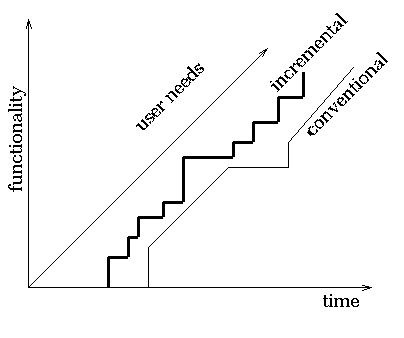
\includegraphics[width=.5\textwidth]{section02/assets/IncrementalModel.png}
\caption[Graphical Illustration of Incremental Prototyping Model]{\label{IncrmentalModel}Graphical Illustration of Incremental Prototyping Model}
\end{figure}

\par Each increment includes the completion of several functional requirements. This project involved seven total increments.  The functional requirements associated with each increment were determined by the sponsor and the developer.  The order in which the requirements for each iteration were determined was dependent upon their general importance and their contribution to the entire system.
\par Functionalities concerning image recognition procedure  and image processing should have a higher priority than others. The increments that occurred in this project are listed below:
\begin{itemize}
\item Increment 1: Graphical User Interface functionalities related to basic user interaction.
\item Increment 2: Image recognition's functionalities related to application interaction.
\item Increment 3: Image perspective functionalities related to application interaction.
\item Increment 4: Enhancing application review and evaluation.
\item Increment 5: System configuration.
\item Increment 6: Writing and executing test cases.
\item Increment 7: Enhancing interactivity of Graphical User Interface.
\end{itemize}}{}\clearpage
\IfFileExists{section03/section}{\section{Design}
\label{sec:Design}

\subsection{Database Design} 
Bmob online database was chosen for the database management system (DBMS) for both the Android application and the web interface because it is a free and open source product. The entity relationship (ER) diagram for the whole project is shown in Figure \ref{ERDiagram}.

\begin{figure}[htb]
\centering
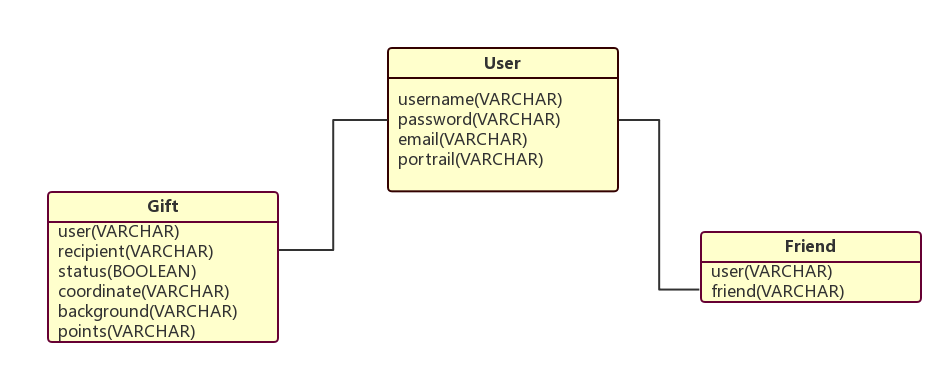
\includegraphics[width=.5\textwidth]{section03/assets/ERDiagram.png}
\caption[Short Caption 2]{\label{ERDiagram}ER Diagram for the project}
\end{figure}

\paragraph{}
All three tables designed for this project are listed in the ER Diagram.
\begin{itemize}
\item The 'User' table will save all the user information. In this table username and email will be unique for each user and this will be verified when users are registered.
\item The 'Friend' table is for saving all friends pairs and both 'user' and 'friend' columns are usernames from 'User' table.
\item The 'Gift' table saves all the gifts information. The 'user' column records the user who sent the gift. The 'recipient' column records the user who will receive the gift. The 'status' column is a boolean type data meaning the gift is found if it is 'true'. The 'coordinate' column is designed to hold the location where the gift was sent. The 'background' column is designed to hold the region picture and the 'points' column is designed to hold the four corners selected by users.
\end{itemize}

\subsection{User Interface Design}
\paragraph{}Following the user interface design principles, especially the accessibility, this user interface is designed to be clear and easy to use. All the parts keep the same color style and try not to use too many colors and fonts so that the user interface is aesthetically pleasing. The main pages are listed below:
\begin{figure}[htb]
\centering
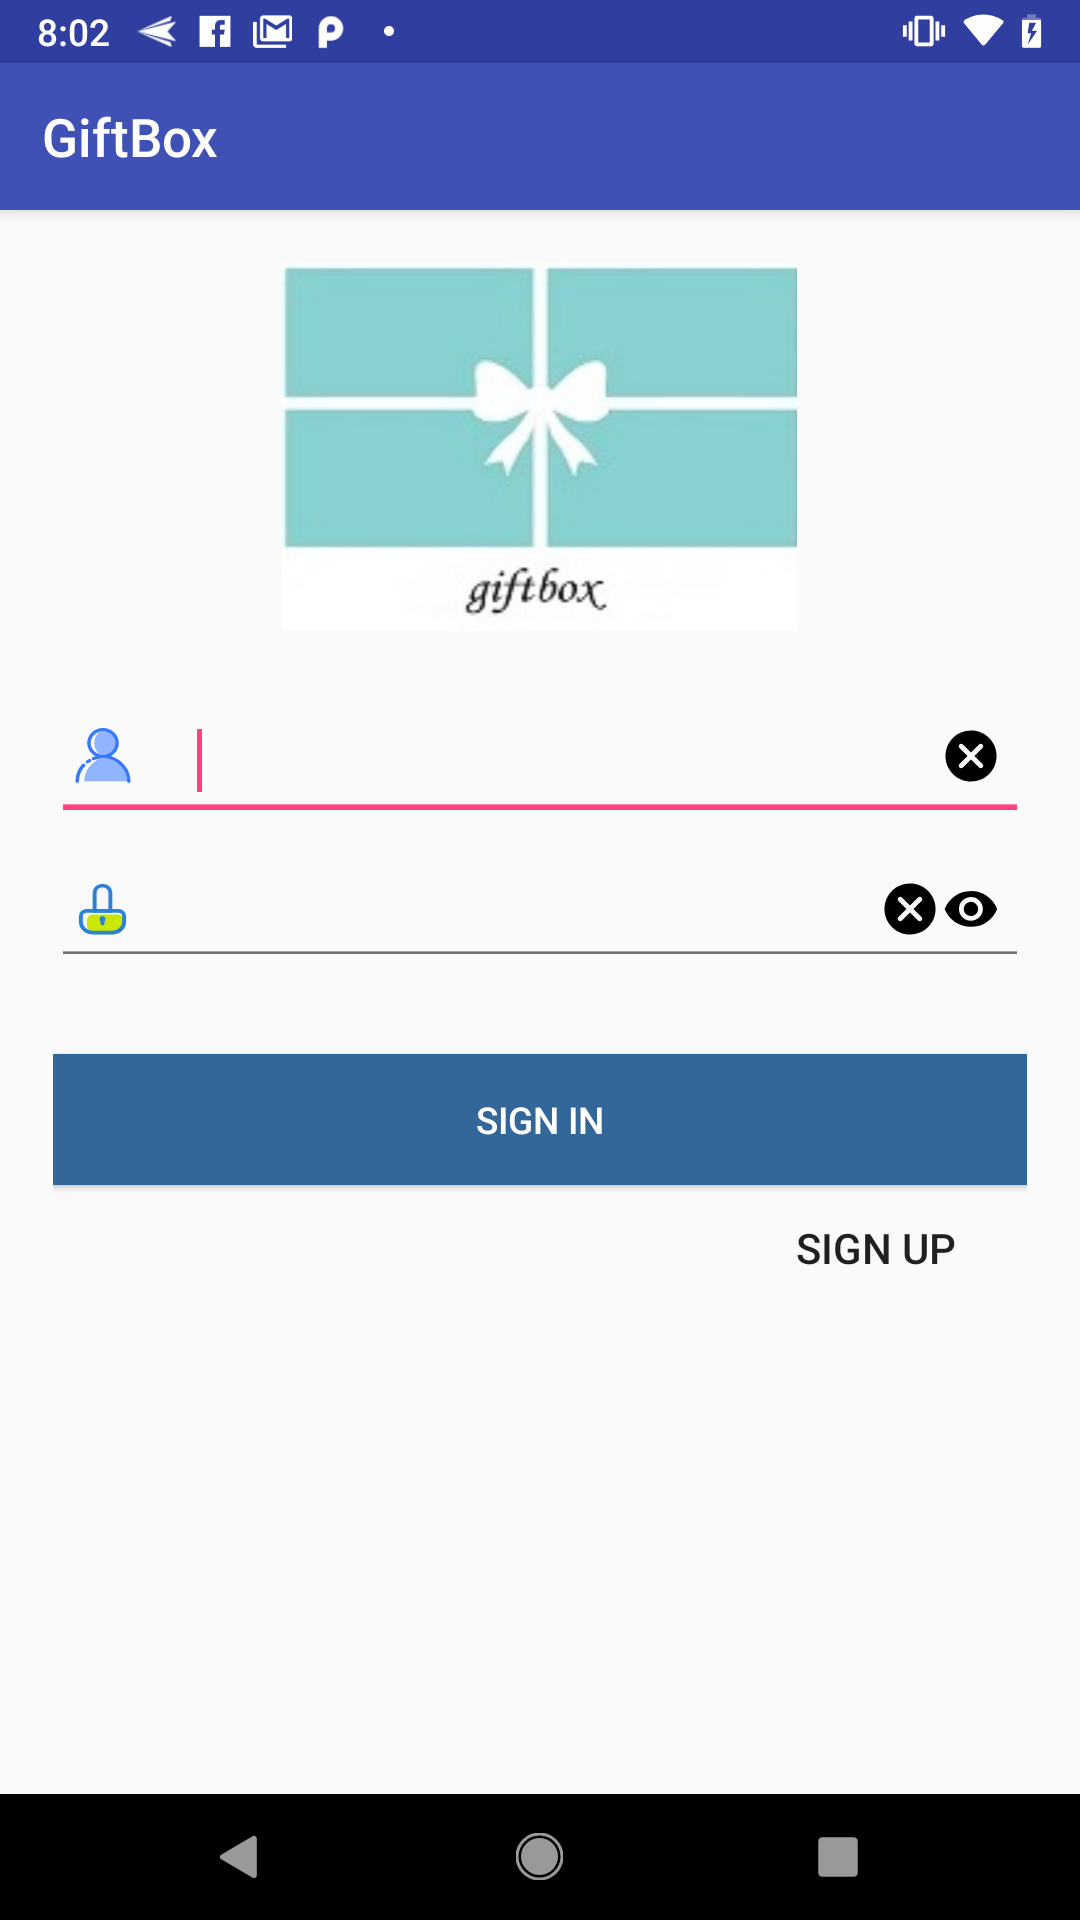
\includegraphics[width=.5\textwidth]{section03/assets/SignIn.png}
\caption[Short Caption 2]{\label{SignInUI}ER Diagram for the project}
\end{figure}
\par The sign in page is shown in Figure \ref{SignInUI}. The logo is designed to show up so that the user will know which application they are using. The user icon and the password icon at the left side of the text field hint the meaning of the two fields to the users. The delete icon and the eye icon at the right side of the text field used another color because they have different functions. Users can use the delete button to delete the whole string they typed in and view the password in plain text or encrypted text. The 'Log In' button is designed to be big to prevent users from making mistakes. 

\begin{figure}[htb]
\centering
\begin{minipage}[t]{0.5\textwidth}
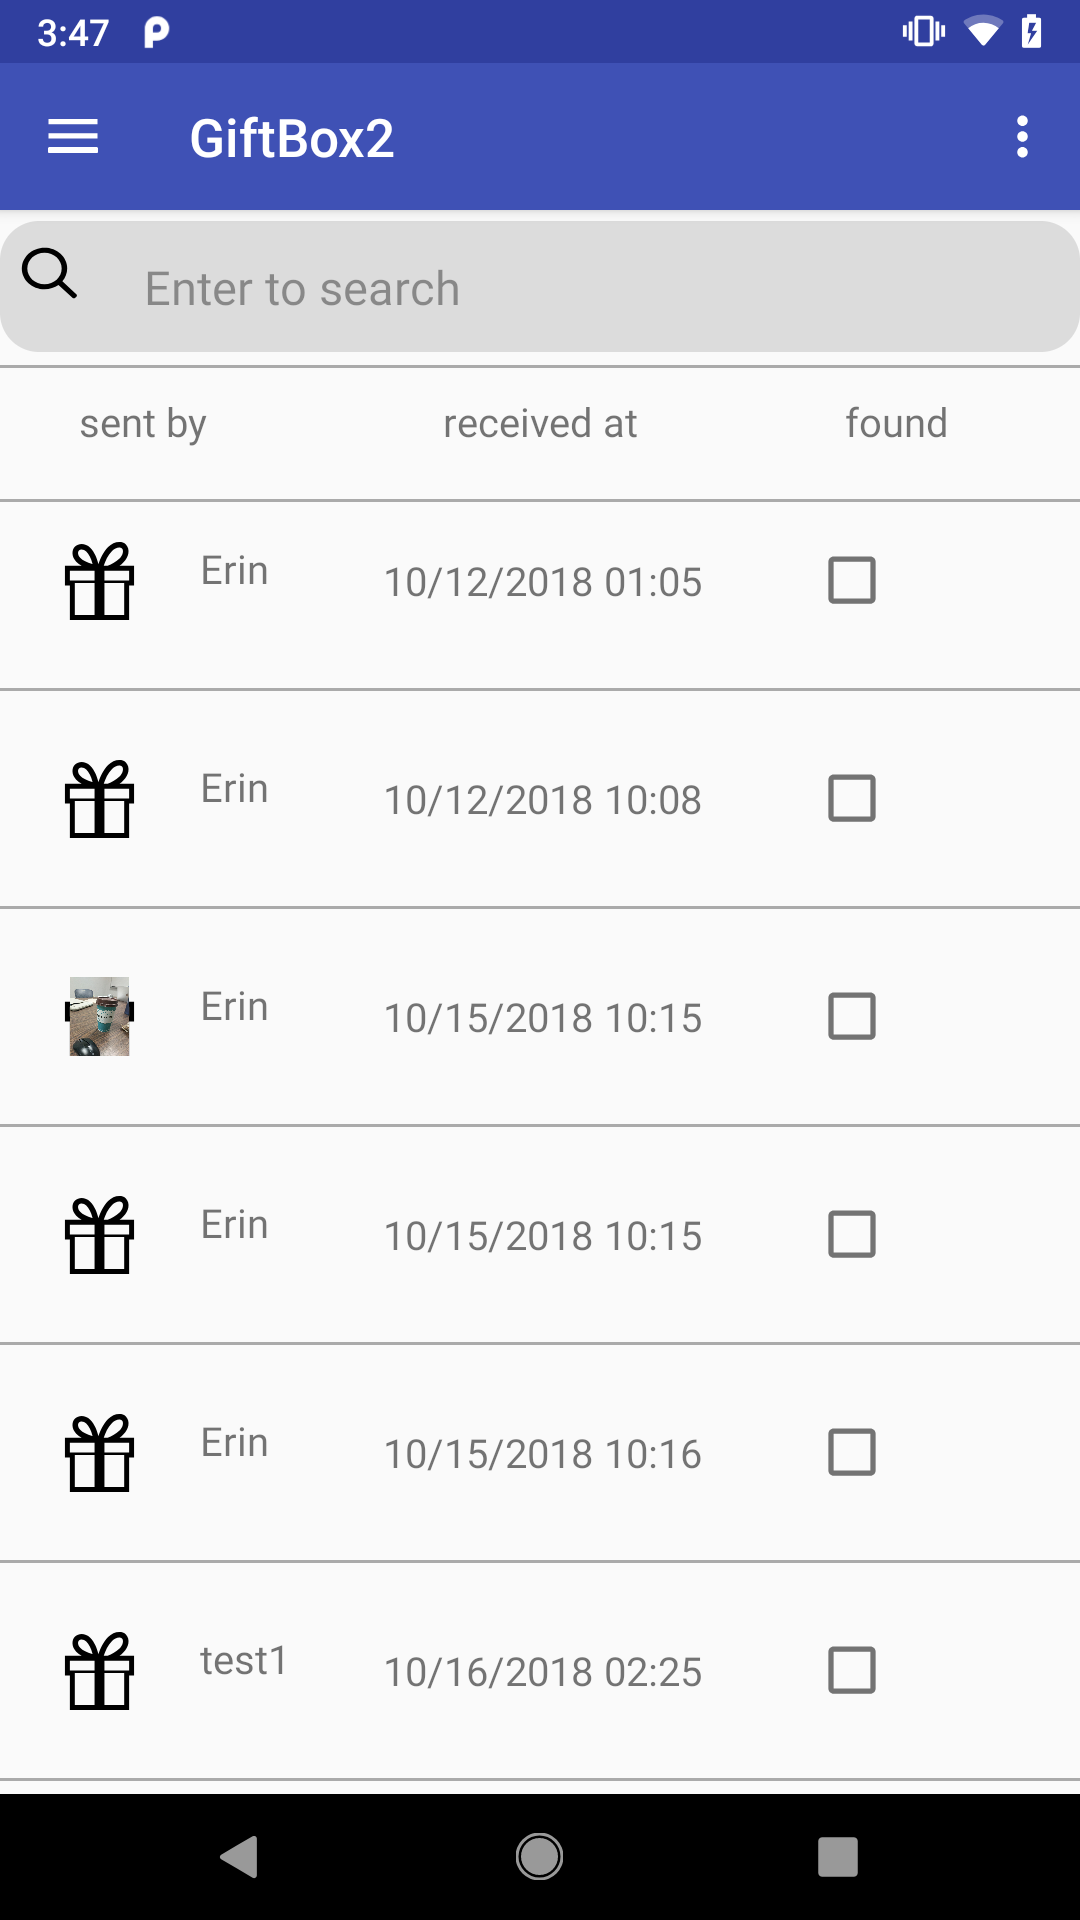
\includegraphics[width=.95\textwidth]{section03/assets/MainPage.png}
\subcaption{\label{GiftsListMainUI}}
\end{minipage}%
\begin{minipage}[t]{0.5\textwidth}
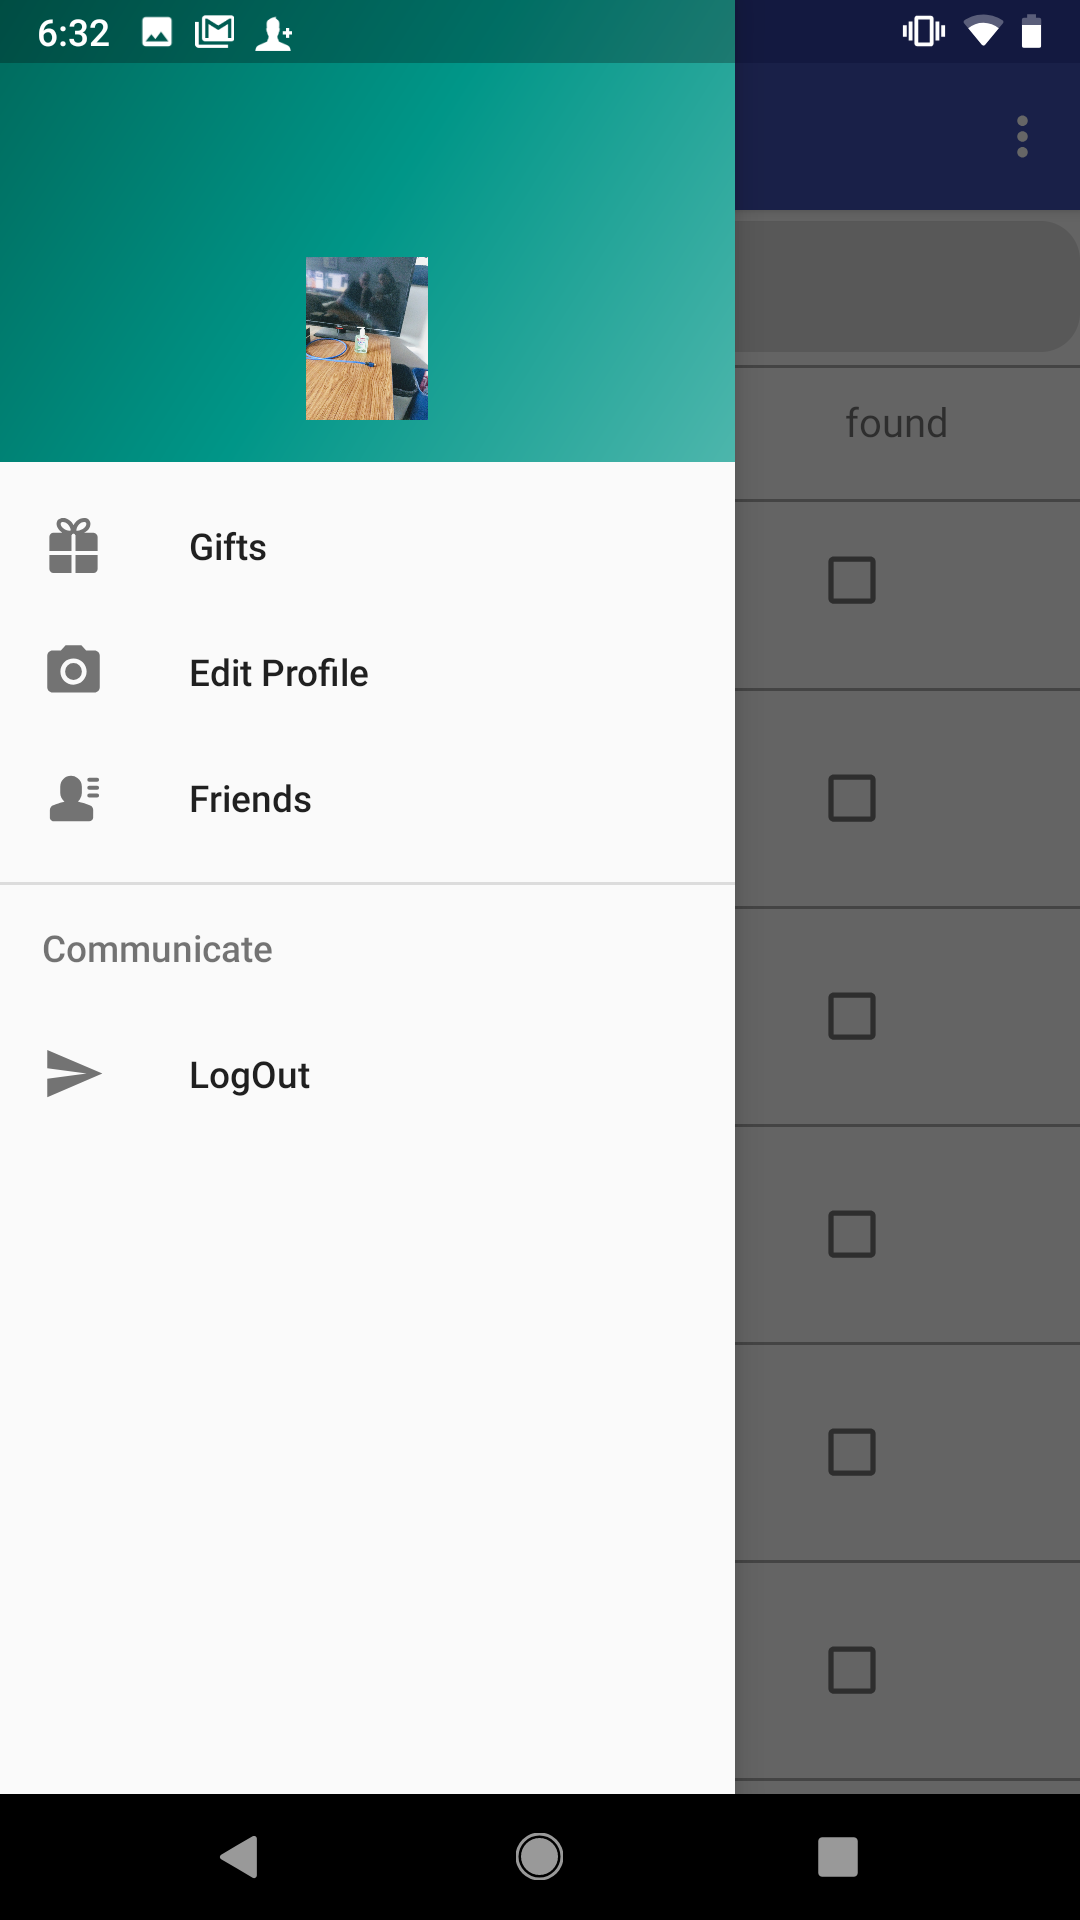
\includegraphics[width=.95\textwidth]{section03/assets/MainPortrait.png}
\subcaption{\label{FunctionsMainUI}}
\end{minipage}%
\caption[Short Caption 2]{\label{MainPageUI}Main page}
\end{figure}
\par The main page is shown in Figure \ref{MainPageUI}. The Figure \ref{GiftsListMainUI} shows the gifts received by the user. The top search field can searched by username. This page also has titles to tell user the meaning of each column. The gift icon was replaced by user portraits later. The found column shows whether or not the gift is found. If the box is checked that means the gift is found.
\par The navigation menu will lead users to other functional pages. Users will see their portraits on the top of this page and will be able to change their portraits by clicking on the profile picture. They can also view their gifts list by clicking on the 'Gifts' button, edit their profile by clicking on the 'Edit Profile' button, view their friends list as shown in Figure \ref{FriendsListUI} by clicking on the 'Friends' button and they will be able to log out from the system by clicking on the 'LogOut' button. 

\begin{figure}[htb]
\centering
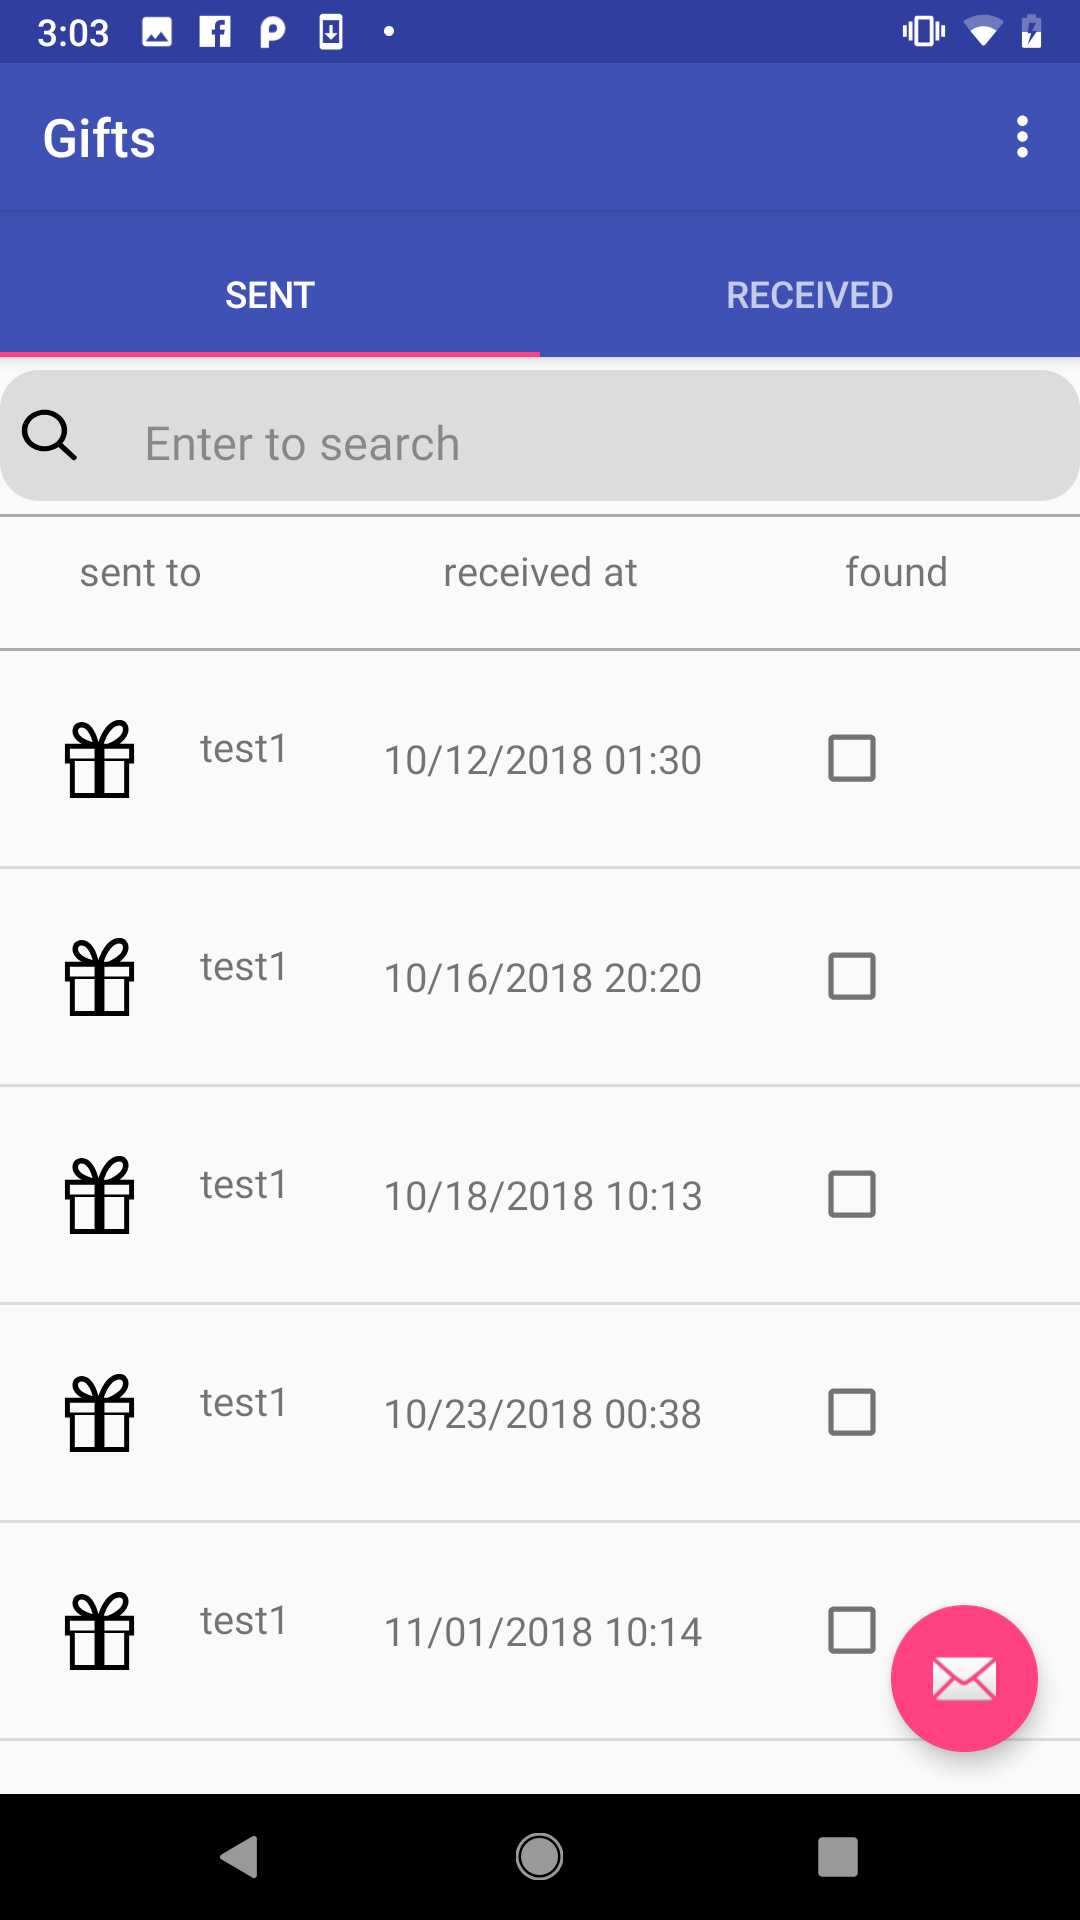
\includegraphics[width=.5\textwidth]{section03/assets/GiftsList.png}
\caption[Short Caption 2]{\label{GiftsListUI}Gifts List page}
\end{figure}
\par Figure \ref{GiftsListUI} is very similar to the main page gifts list but in this page users will be able to see not only received gifts but also sent gifts ordered by time stamp. For the sent gifts, users will be able to see if this gift is found or not by clicking on the gift. For the received gifts, they can only view found gifts and begin to find unfound gifts by clicking on the gift. 


\begin{figure}[htb]
\centering
\begin{minipage}[t]{0.5\textwidth}
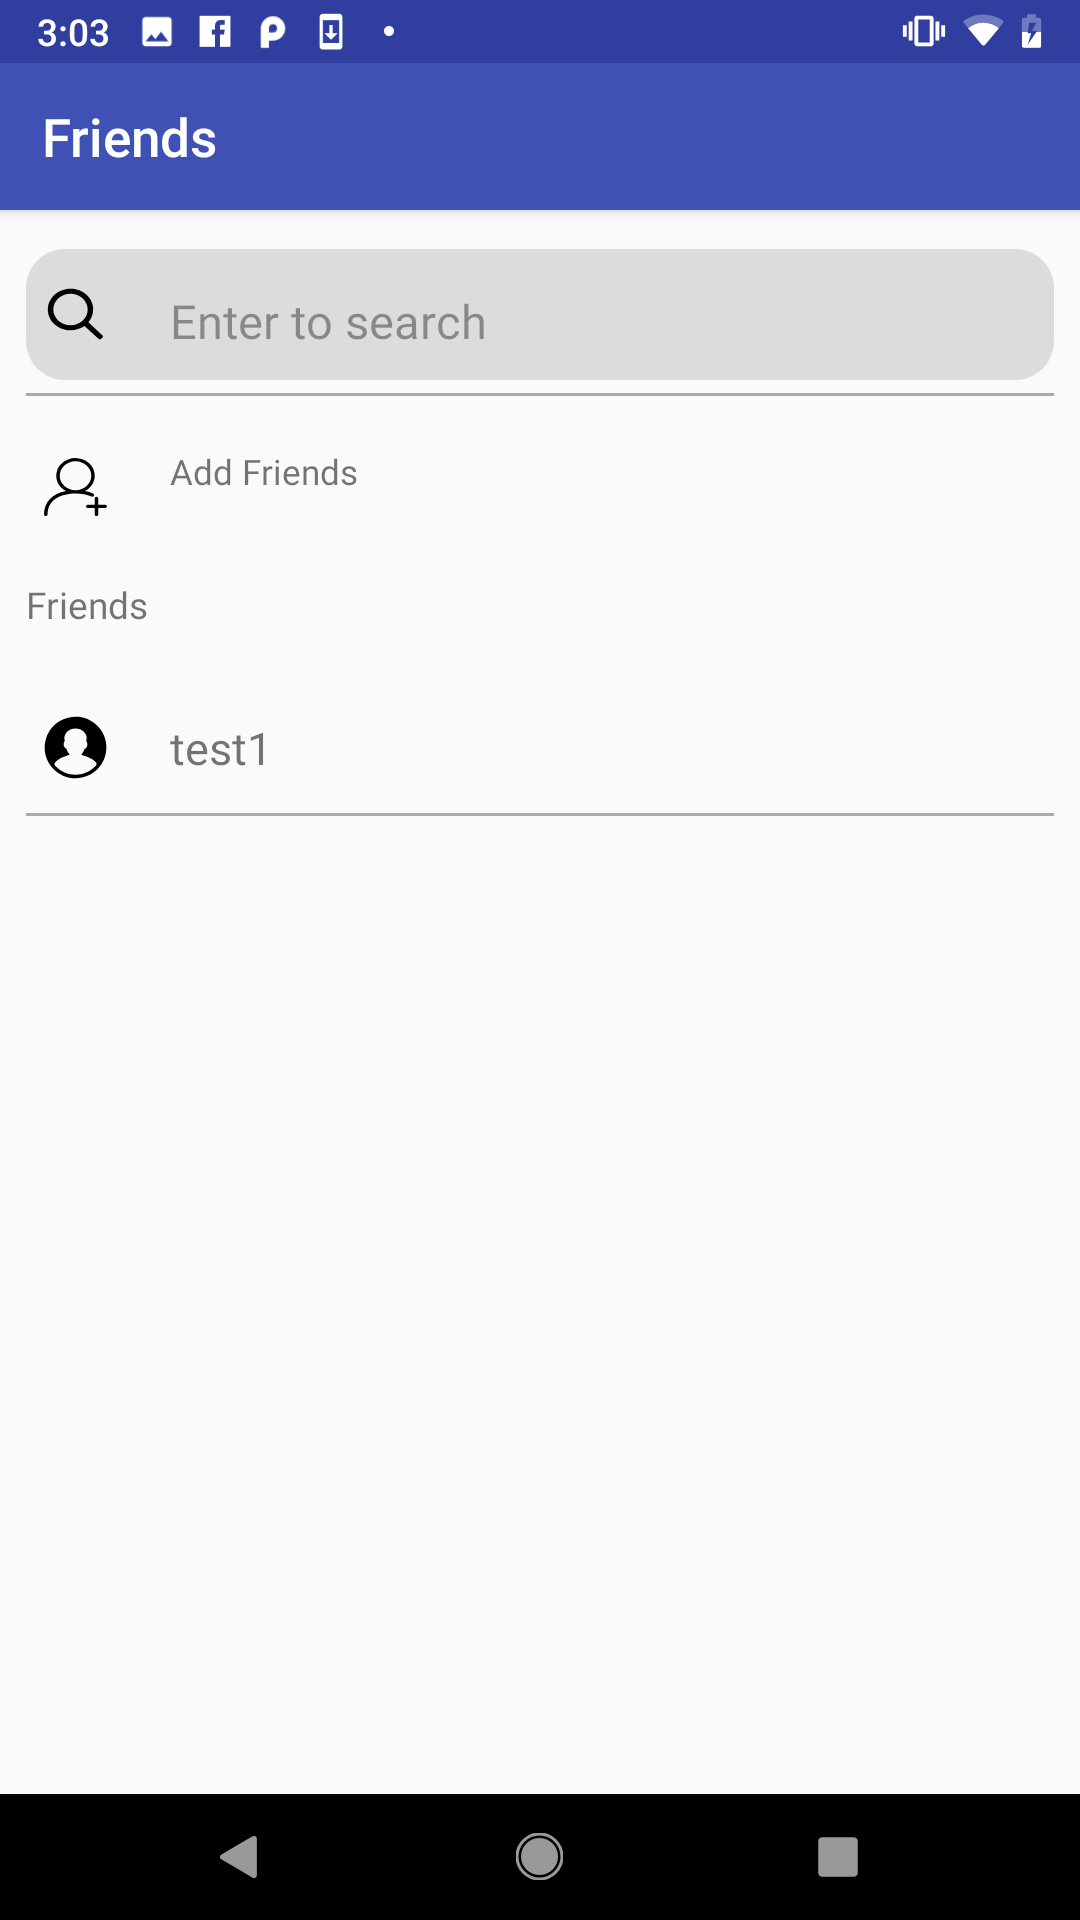
\includegraphics[width=.95\textwidth]{section03/assets/FriendsList.png}
\subcaption{\label{FriendsListUI}}
\end{minipage}%
\begin{minipage}[t]{0.5\textwidth}
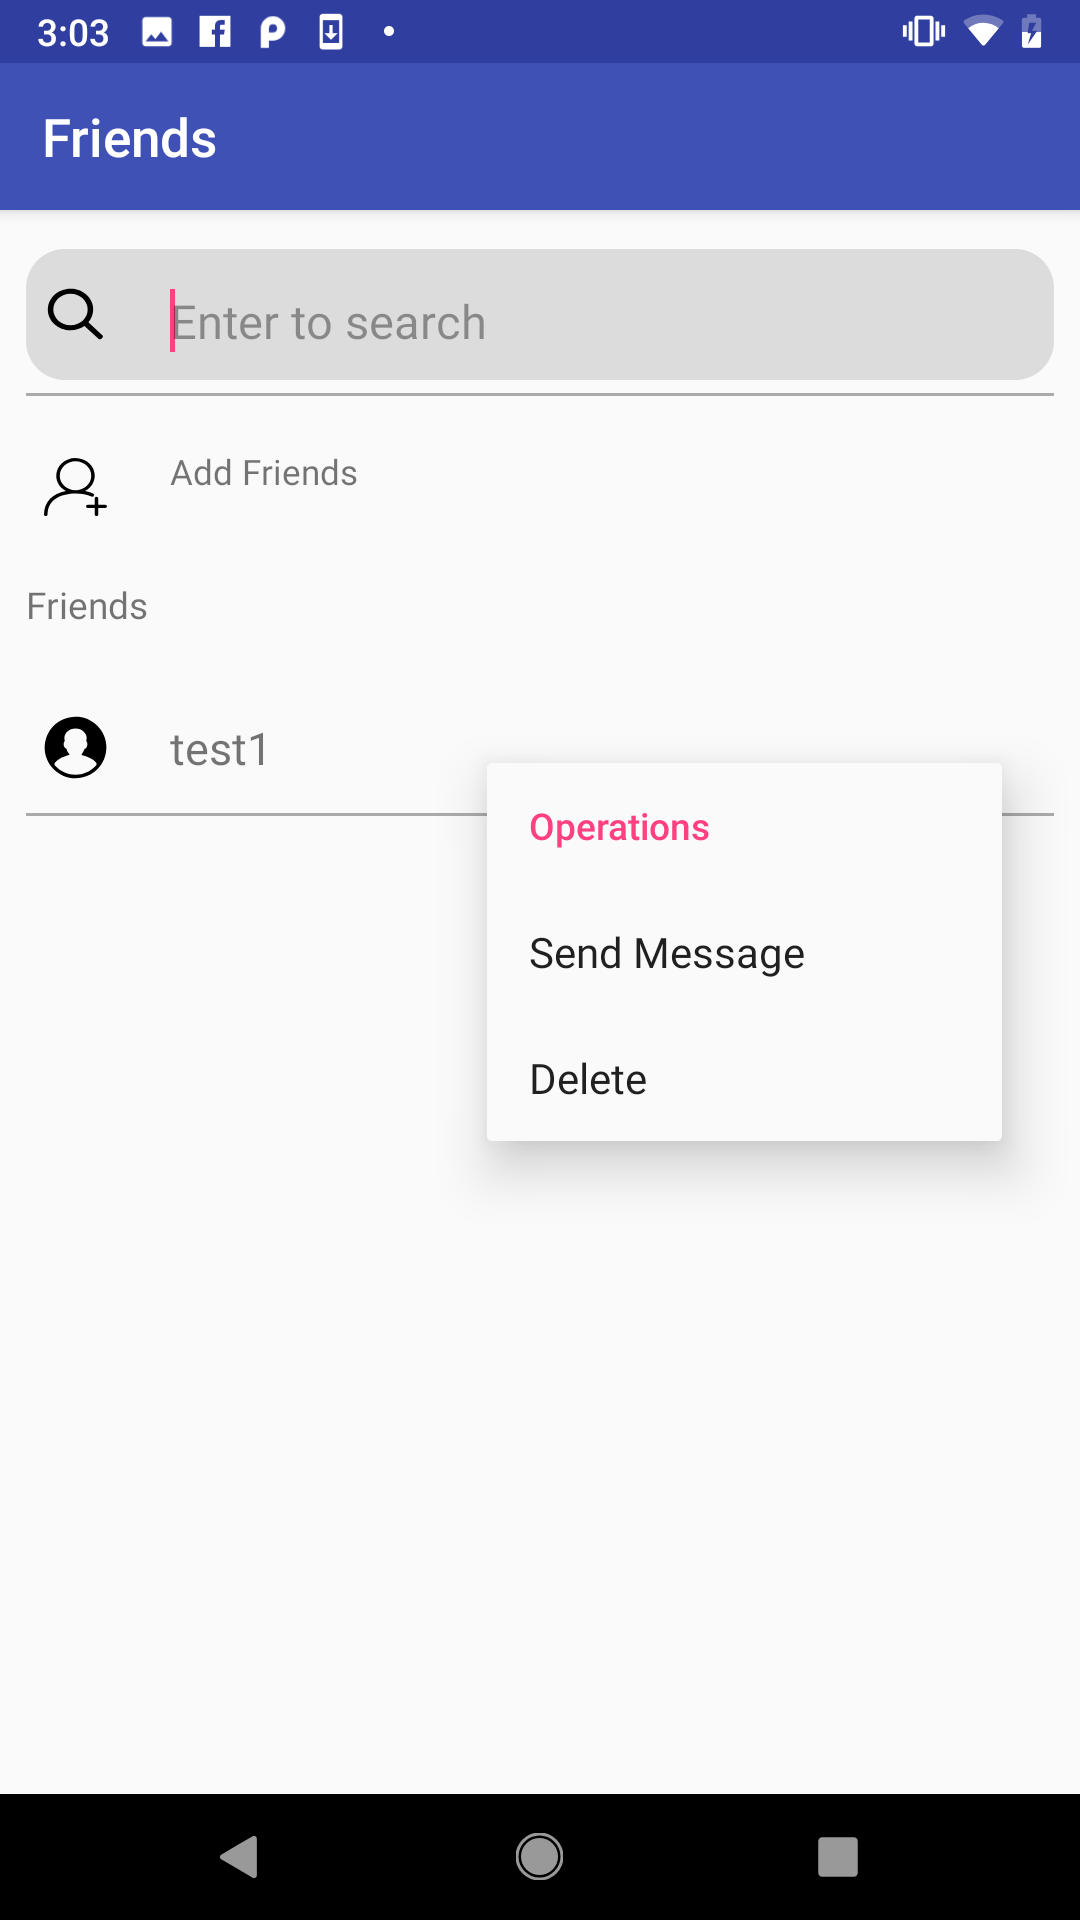
\includegraphics[width=.95\textwidth]{section03/assets/FriendsListAction.png}
\subcaption{\label{FriendsListActionUI}}
\end{minipage}%
\caption[Short Caption 2]{\label{WholeFriendsListUI}Friends List page}
\end{figure}

\par As shown in Figure \ref{WholeFriendsListUI}, the friends list is another important page for this application. To convenience users, the search field can let users search their friends if their friends list is too long. Users can also add friends by clicking on the 'Add Friends' button. The friends list is shown below. Users can get further functions by long clicking on friends' names, as shown in Figure \ref{FriendsListActionUI}. 

\begin{figure}[htb]
\centering
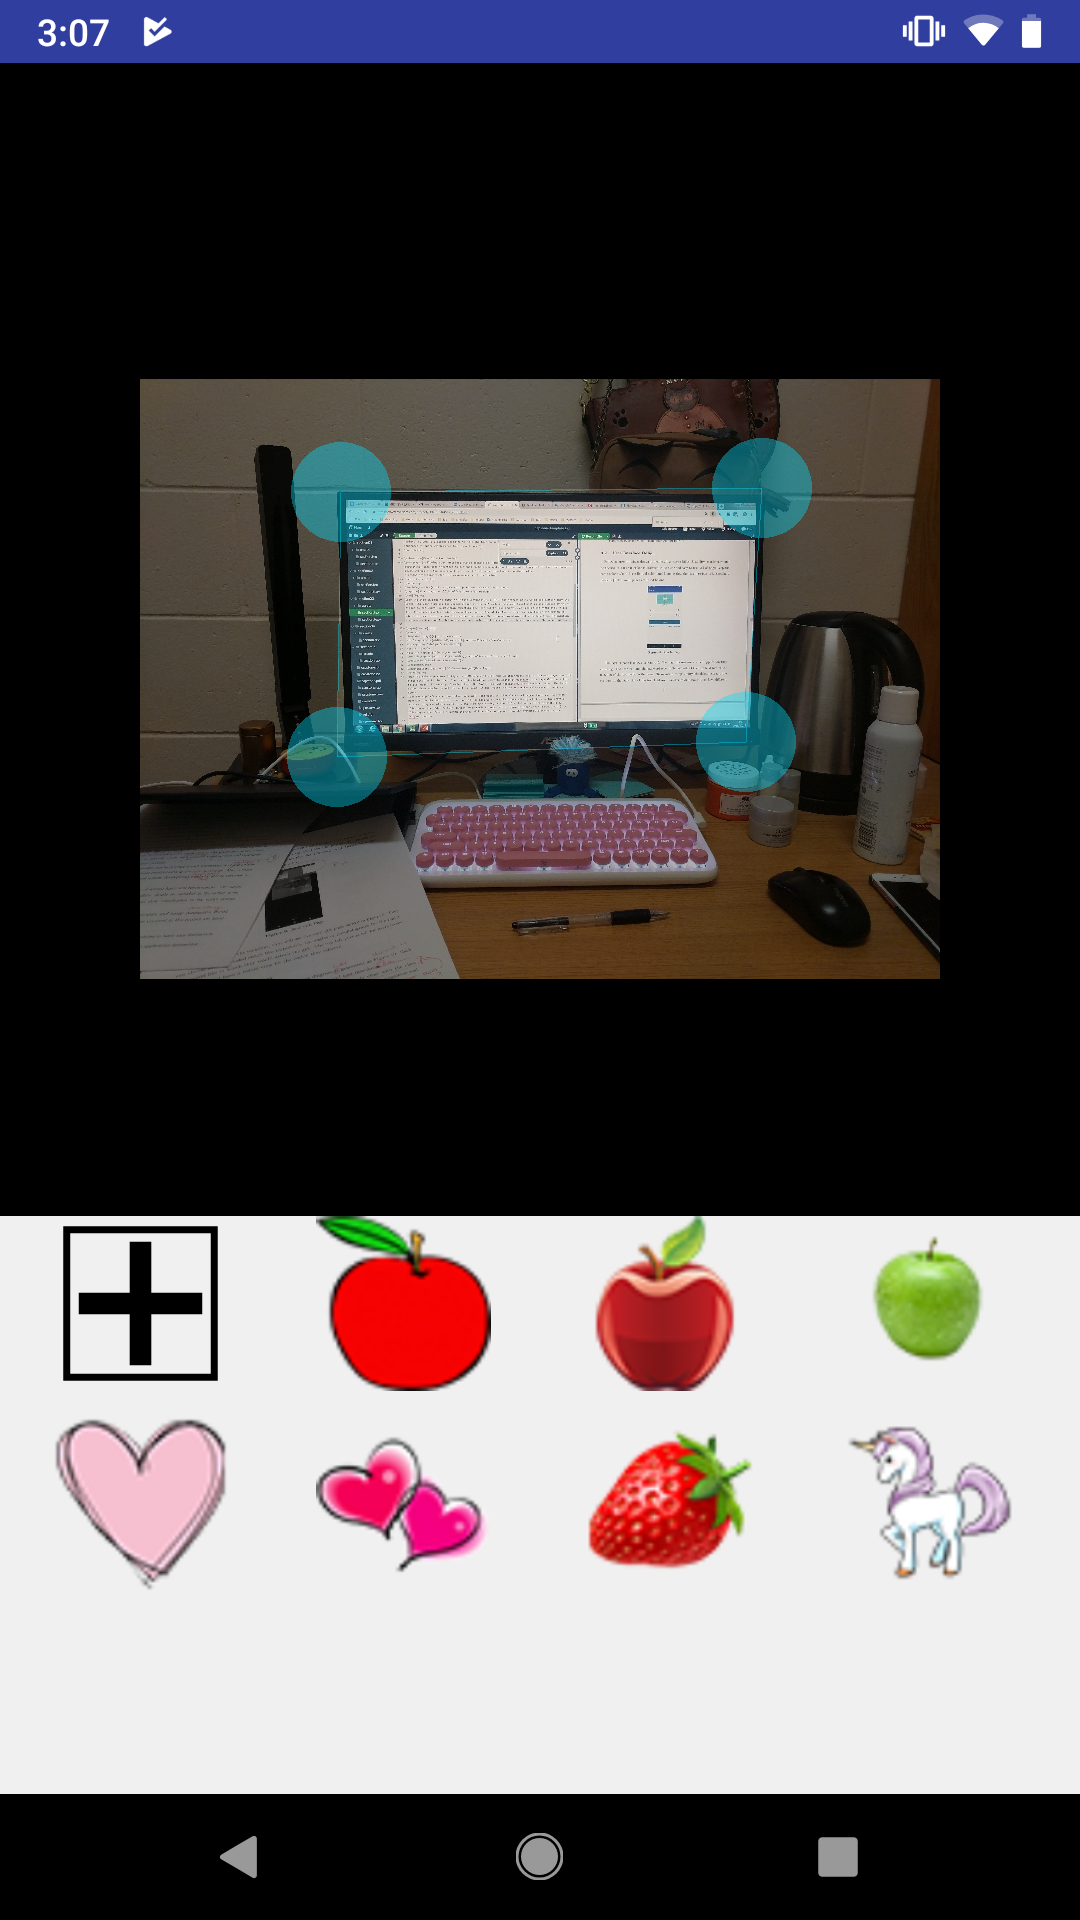
\includegraphics[width=.5\textwidth]{section03/assets/SendGift.png}
\caption[Short Caption 2]{\label{SendGiftUI}Send Gift Page}
\end{figure}
\par After users choose the recipient, they will see the send gift page shown in Figure \ref{SendGiftUI}. They can choose any four sided shape like trapezoids, rectangles or parallelograms for the region they would like in which they would attach the gift.

\subsection{Architecture Design}
\paragraph{}Based on the functional requirements, the class diagram is generated as Figure \ref{ClassDiagram}. Each class is correspond to one or more functional requirements and user interfaces.
\par As we can see, the basic user interaction related class is already clear with the class diagram. So we are just going to explain classes and functions about image recognition and navigation.

\begin{figure}[H]
\centering
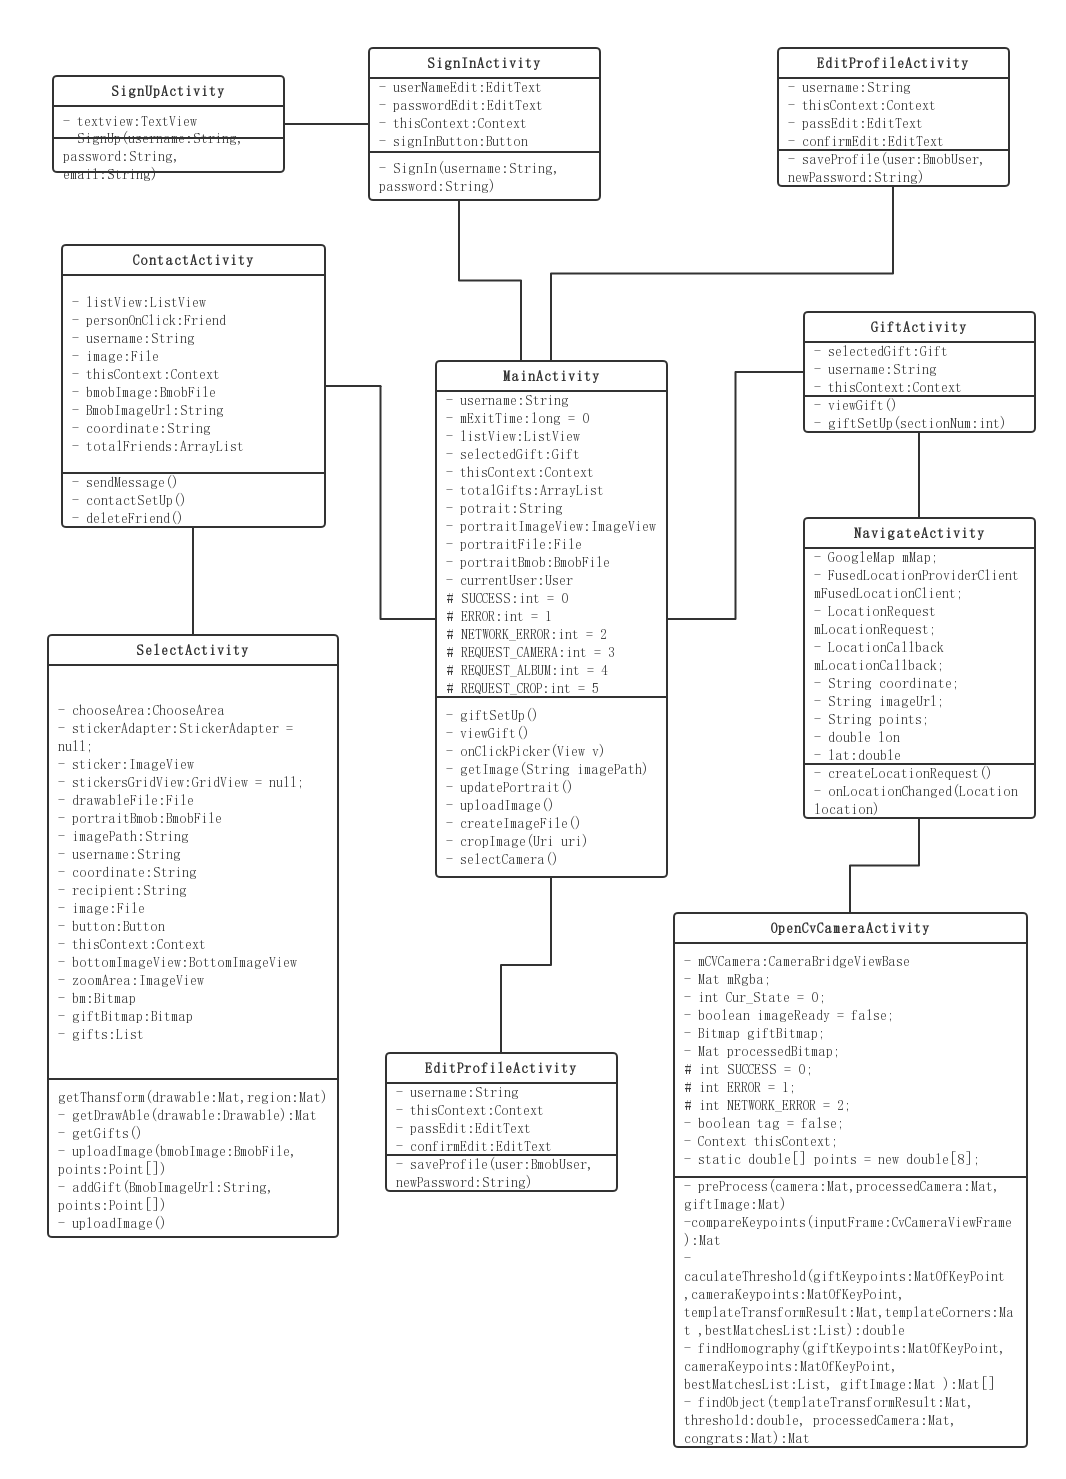
\includegraphics[width=.8\textwidth]{section03/assets/ClassDiagram.png}
\caption[Short Caption 2]{\label{ClassDiagram}Class Diagram}
\end{figure}
\par The 'ContactActivity' is mainly related to the user interface shown in Figure \ref{FriendsListUI}, users will be able select their recipient and the information will be taken to 'SelectActivity' by an intent and then the system camera will be called to get the background image, the 'chooseArea' attribute is an instance of helper class 'ChooseArea' to let the users choose the region. After that, the gift will fit in the region by 'getTransform' method and 'addGift' method will save all the information to the database.
\par The receiving process is explained as follow. The 'GiftActivity' is designed to show the gift list which shown in Figure \ref{GiftsListUI}, when users click on a not found gift they will go to 'NavigationActivity'. The 'NavigationActivity' is designed to manage user locations and Google Map activities. Users will be able to see their location on the map and the gift location will be marked in a red point. When user found where the gift locates, the real-time image recognition will start. The camera capture images will compare with the database saved background image. The 'preProcess' method is used to download the database saved background image and resize the camera capture image. The 'compareKeypoints' method calculates the keypoints in two images and find the matches. The 'findHomography' method will use the matches found before to generate the homography and perform a perspective transformation on the template image to correct the image to get the region in camera image. But this method cannot always get the correct result, so the 'caculateThreshold' method calculate the value of the number of keypoints not in selected region divide the number of keypoints in detected region, this value will be later used as a threshold to determine if the region we found is good. At last, the 'findObject' method will get the final detected region and show the gift on it.


}{}\clearpage

%% BIBLIOGRAPHY
\section{Bibliography}
\label{sec:bibliougraphy}
\clearpage


%%% APPENDICES
\section{Appendices}
\label{sec:appendices}
\clearpage

\end{document}
